%%%Dokumentklasse
\documentclass[12pt,twoside,fleqn]{book}

\usepackage{graphicx}
\usepackage{wrapfig}
\graphicspath{ {img/} }	
\usepackage[a4paper,width=150mm,top=25mm,bottom=25mm]{geometry}
\usepackage{calc}
\usepackage{amsmath}
\usepackage{amssymb}
\usepackage{amsfonts}           % einige weitere Sonderzeichen
\usepackage{subfigure}          % erlaubt das Anordnen von Bildern nebeneinander mit einzelnen Bildunterschriften
                                % einfacher, als mit Tabellen und Boxen zu arbeiten
\usepackage{ngerman}
\usepackage{bibgerm}            % Stylefile für deutsche Literaturstellenangabe
\usepackage[T1]{fontenc}        % saubere Trennung von Wörtern mit Umlauten
\usepackage[utf8]{inputenc}   % direkte Eingabe von Umlauten
\usepackage{fancyhdr}
\usepackage{colortbl}
\usepackage{hhline}
\usepackage[bf]{caption}
\usepackage[noadjust]{cite}     % erlaubt Zeilenumbruch innerhalb von Zitierungen, Option noadjust verhindert
                                % automatische Leerzeichen um die Referenz, was am Zeilenanfang zu Problemen führt
\usepackage{hyperref}           % erlaubt die Nutzugn von \url
\usepackage{code}          % Style vom Fachgebiet NIKR für Pseudocode-Darstellung

%\usepackage{pdfpages}
\usepackage[xindy,toc]{glossaries}
\sloppy

\usepackage{placeins}
% === Längen und Abstände ==================================================

% horizontales Layout
\setlength{\oddsidemargin}{0.2in}
\setlength{\evensidemargin}{0.0in}
\setlength{\textwidth}{\paperwidth - 2.2in}

% vertikales Layout
%\setlength{\topskip}{0.0cm}
\setlength{\headheight}{15.1pt}
%\setlength{\headsep}{0.0cm}
\setlength{\topmargin}{0.0cm}
\setlength{\footskip}{0.6in}
\setlength{\textheight}{\paperheight - 2.0in}
\addtolength{\textheight}{-1.0\headheight}
\addtolength{\textheight}{-1.0\headsep}
\addtolength{\textheight}{-1.0\footskip}

% Zeilenabstand
\renewcommand{\baselinestretch}{1.5}

\setlength{\topsep}{0.3cm}
\setlength{\mathindent}{1.0cm}
\setlength{\parindent}{0.0cm}

% === Bildunterschrift ========================================================

\renewcommand{\captionfont}{\small}
\newcommand{\NIcaption}[2]{\caption[#1]{#1\protect\\ \emph{#2}}}
\setcaptionmargin{0.75cm}
%\renewcommand{\topfraction}{0.95}
%\renewcommand{\textfraction}{0.05}
%\renewcommand{\textfloatsep}{1.0cm}

% === Seitenstil ==============================================================

\pagestyle{fancy}
\fancyhead[ER]{\itshape\leftmark}
\fancyhead[OL]{\itshape\rightmark}
\fancyhead[EL,OR]{\thepage}
\fancyfoot[ER,OL]{\small \invNumText}
%\fancyfoot[ER,OR]{\invNumText}
%\fancyfoot[EL,OL]{\myName}
\fancyfoot[EC,OC]{}
\renewcommand{\headrulewidth}{1pt}
\renewcommand{\footrulewidth}{0.4pt}

\fancypagestyle{plain}{
\fancyhead[ER]{\itshape\leftmark}
\fancyhead[OL]{\itshape\rightmark}
\fancyhead[EL,OR]{\thepage}
\fancyfoot[ER,OL]{\small \invNumText}
%\fancyfoot[ER,OR]{\invNumText}
%\fancyfoot[EL,OL]{\myName}
\fancyfoot[EC,OC]{}
\renewcommand{\headrulewidth}{0.4pt}
\renewcommand{\footrulewidth}{0.4pt}}

% von den nachfolgenden Bl�cken bitte den richtigen
% ausw�hlen, die anderen auskommentieren/l�schen

% -------- Diplom ----------
%\newcommand{\Degree}{{Diplom}}
%\newcommand{\DegreeName}{{Diplominformatiker}}     % je nach Fachrichtung ausw�hlen
%\newcommand{\DegreeName}{{Diplomingenieur}}
%\newcommand{\invNum}{{xxx-xxx-xxx}}                % wird vom Pr�fungsamt vergeben    
%\newcommand{\invNumText}{{Inv.-Nr: \invNum}}
%\newcommand{\invNumTextLong}{{Inventarisierungsnummer: \invNum}}
%\newcommand{\inputthesen}{\chapter*{Thesen}
\thispagestyle{empty}

Die Thesen sollen die wesentlichen Aussagen der Diplomarbeit in pr�gnanter Form
darstellen.

\begin{itemize}
    \item Zur L�sung des St�rmerproblems der deutschen
    Fu�ball-Nationalmannschaft ist der Einsatz zuverl�ssiger humanoider
    Roboter dringend notwendig.
    \item Gegenw"artig existierende Konzepte und L"osungen sind nicht in der Lage,
    die komplexen Anforderungen, die das Szenario Fu�ballspiel an den Roboter
    stellt, zu erf"ullen.
    \item Das Verfahren ABC "uberwindet die Einschr"ankungen der Methode xyz und
    erm"oglicht einem Roboter die intuitive Erfassung der Spielsituation mittels
    optischer Sensorik. 
    \item Durch die Weiterentwicklung des Schuss-Systems RoboFoot werden
    deutlich h"ohere Ballgeschwindigkeiten erzielt, was zu einer Erh"ohung der
    durchschnittlichen Erfolgsrate beim Torschuss f"uhrt.
    \item Es wurde experimentell nachgewiesen, dass der Roboter-Fu�baller
    Robario seinen menschlichen Konkurrenten in der Chancenverwertung um ca. 112\%
    �berlegen ist.
\end{itemize}

  \vspace*{1cm}

  \begin{sloppy}
  \hspace{2em}\begin{tabular}{lp{10cm}}
    \multicolumn{2}{l}
    {Ilmenau, \finishdate \hspace{5.5cm} \dotfill}\\
    \multicolumn{2}{l}
    {\hspace{8,5cm}Max Mustermann} \\
  \end{tabular}
  \end{sloppy}
\vfill
}

% -------- Bachelor ----------
\newcommand{\Degree}{{Bachelor}}
\newcommand{\DegreeName}{{Bachelor of Engineering}}
\newcommand{\invNumText}{{}}
\newcommand{\invNumTextLong}{{}}
\newcommand{\inputthesen}{}

% -------- Master ----------
%\newcommand{\Degree}{{Master}}
%\newcommand{\DegreeName}{{Master of Science
%\newcommand{\invNumText}{{}}
%\newcommand{\invNumTextLong}{{}}
%\newcommand{\inputthesen}{}

\newcommand{\myName}{{Elias Marks}}   % der eigene Name
\newcommand{\finishdate}{{14.03.2016}}   % Datum der Abgabe

\graphicspath{{img/}}                    % Suchpfad (Unterverzeichnis) f�r eingebundene Grafiken


\newcommand{\quotes}[1]{``#1''}
%\makeglossaries
\makenoidxglossaries

\newglossaryentry{scale-space}
{
  name={scale-space},
  description={}
}

\newglossaryentry{scale}
{
  name={scale},
  description={},
  plural={scales}
}

\newglossaryentry{octave}
{
  name={octave},
  description={},
  plural={octaves}
}

\newglossaryentry{Online-System}
{
  name={Online-System},
  description={},
  plural={Online-Systeme}
}


\begin{document}
	
    \frontmatter
    \pagestyle{empty}
    % === Titelblatt ==============================================================

\begin{titlepage}
\large
%\hspace{0.2cm}
\begin{center}
{\bf Hochschule Heilbronn}\\
Robotik und Automation\\
\end{center}

\hspace{0.2cm}

\begin{minipage}{\textwidth}
\begin{center}

\includegraphics[width=0.4\textwidth]{hhn_logo.png}

\end{center}
\end{minipage}

\begin{center}
\vspace{0.8cm}
{\Large\bfseries Analyse verschiedener Merkmalsextraktionsverfahren zur Objekt-Klassifizierung\\}
\vspace{0.8cm}
\end{center}

\begin{table}[ht]
\begin{tabular*}{\linewidth}{p{0.5\linewidth} p{0.5\linewidth}}
Name & Elias Marks\\
Matrikelnummer & 184949\\
Anschrift & Max-Planck-Str. 27\\
& 74081 Heilbronn \\
&\\
Betreuer & Prof. Dr. Dieter Maier\\
Email & dieter.maier@hs-heilbronn.de\\
Telefon & +49 7131 504 399\\
Anschrift & Hochschule Heilbronn\\
& Max-Planck-Str. 39\\
& 74081 Heilbronn \\
%\multicolumn{2}{l}{Verantwortlicher Hochschullehrer:}\\
%	  & Prof.~Dr.~H.-M.~Gro"s, FG Neuroinformatik und Kognitive
%	  Robotik\\[2cm]

\end{tabular*}
\end{table}


\vspace{1.0cm}
\begin{sloppy}
\begin{tabular}{lp{10cm}}
\multicolumn{2}{l}
{Heilbronn, \finishdate \hspace{5.5cm} \dotfill}\\
\multicolumn{2}{l}
{\hspace{8,5cm} \myName} \\
\end{tabular}
\end{sloppy}
\end{titlepage}
    \setcounter{page}{0}
    \tableofcontents
    \mainmatter
    \setcounter{page}{1}
    \pagestyle{plain}

    \chapter{Einleitung}
\section{Motivation}

Die Bilddatenverarbeitung gewinnt in unserem technologischem Zeitalter immer mehr an Bedeutung. 
Durch die Verbreitung der Automatisierung in den meisten industriellen und sozialen Umfeldern werden immer neue und effizientere Methoden zur Datenverarbeitung benötigt.
Eine der größten Herausforderungen bei Autonomen Systemen ist die Erfassung der Umgebung um Interaktionen mir dieser, oder kollisionsfreihe Bewegungen zu ermöglichen. 
Zu diesem Zweck werden unter anderem Kameras verwendet.
Diese haben den Vorteil dass sie für ein sehr breites Spektrum an Aufgaben einsetzbar sind da sie eine enorme Menge an Daten sammeln.
Dies hat jedoch zur Folge dass sehr komplexe Algorithmen benötigt werden um die relevanten Informationen, wie die Art oder Position eines Objekts, zu extrahieren.
Als die ersten Steine des heutigen Wissens in diesem Bereich gelegt wurden war die Leistungsfähigkeit der Computer das größte Problem.
Da die Entwicklung schnellerer und günstigerer Recheneinheiten (Prozessoren und Grafikkarten) seit dem sehr große Schritte gemacht hat und weiter machen wird, sind der Verbreitung dieser Technologie immer weniger Grenzen gesetzt.
Außerdem steigt auch die Verbreitung von Handys mit äußerst leistungsstarken Kameras immer mehr und ermöglicht somit neue Anwendungsbereiche dieser Technologie im Alltag.

\section{Untersuchte Algorithmen}

Es gibt verschiedene Ansätze der Bildverarbeitung, auch abhängig von dem voraussichtlichen Anwendungsgebiet.
Neben dem Morphologischen und dem neuesten Ansatz des Deep Learnings wird vor allem die Merkmalsbasierte Bildverarbeitung genutzt.
Dieser besteht besteht in der Bestimmung von Punkten im Bild die bei möglichst vielen Lichtverhältnissen und aus unterschiedlichen Blickwinkeln wiedererkannt werden können.
Durch die Anordnung dieser lokalen Merkmale kann ein Objekt anhand einer Datenbank aus solchen Mustern wiedererkannt und lokalisiert werden.
Zu dieser Sparte der Bildverarbeitung gehören unter anderen die in dieser Arbeit analysierten Algorithmen.
Die Einführung des \emph{Scale-invariant feature transform} (SIFT) war ein sehr großer Schritt in der Entwicklung dieses Bereichs und ermöglichte somit die Verbreitung der Bildverarbeitung in industriellen Umgebungen.
Die anderen hier untersuchten Algorithmen, \emph{SURF} und \emph{ORB}, sind mehr oder weniger eine Ableitung von \emph{SIFT} und sind vor allem ein versuch die Kosten der Berechnung zu mindern um diese Technologie echtzeitfähig zu machen und den Einsatz auf weniger performanten Geräten zu ermöglichen.


    \chapter{Inhalt}

Im laufe dieser Arbeit wurden verschiedene Algorithmen zur lokalen Merkmalsextraktion und Deskriptor Berechnung getestet und ausgewertet.
Das Ziel ist hierbei Merkmale zu finden die so gut wie möglich folgenden Ansprüchen genügen und somit als stabil bezeichnet werden:
\begin{itemize}
\item \emph{Skaleninvarianz}: Unabhängigkeit von der Größe auf dem Bild (Distanz zur Kamera)
\item \emph{Rotationsinvarianz}: Merkmale können trotz einer Rotation erkannt werden
\item \emph{Beleuchtungsinvarianz}: Ermöglicht Erkennung der Merkmale bei verschiedenen Lichtverhältnissen
\item \emph{Blickwinkelunabhängigkeit}: Unabhängigkeit von der Position aus der das Objekt aufgenommen wird
\end{itemize} 

\section{SIFT}

Die "Scale Invariant Feature Transform" ist bis heute eine der erfolgreichsten Methoden zur lokalen Merkmalsextraktion. Sie wurde 1999 von David Lowe vorgestellt und ist von der Objekterkennung im menschlichen Gehirn inspiriert.

\subsection{Merkmalsextraktion}

Aus dem zu untersuchenden Bildes wird als erstes der sogenannte \Gls{scale-space} berechnet.

\begin{figure}[h]
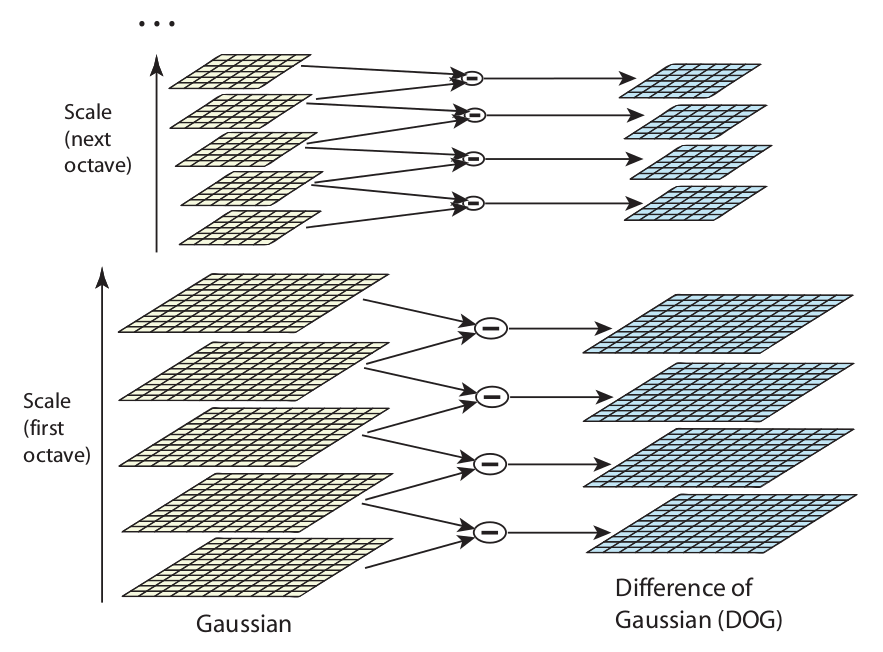
\includegraphics[width=0.6\textwidth]{scale_space.png}
\centering
\end{figure}
Hierzu wird das Bild mit einem Gauss-Kernel wiederholt geglättet um die \Glspl{scale} der ersten \Gls{octave} zu erstellen.
Um die Gaussgeglätteten Bilder $ L (x, y, \sigma ) $ zu erhalten wird der Gauss-Kernel 
\begin{equation}
G(x, y, \sigma) = \frac{1}{2\pi\sigma^{2}}e^{-(x^{2}+y^{2})/2\sigma^{2}}
\end{equation}
 mit dem Ursprungsbild $ I(x, y) $ gefaltet:
\begin{equation}
L(x, y, \sigma) = G(x, y, \sigma)\ast I(x, y)
\end{equation}
Hiermit werden schrittweise immer mehr kleine Merkmale entfernt, was dazu führt dass größere Merkmale and Bedeutung gewinnen.
Die Breite der Gaussfunktion mit der zwei benachbarte \Glspl{scale} berechnet werden, haben das konstante Verhältnis $ k $, hierdurch sind die \Glspl{scale} im \Gls{scale-space} equidistant in Bezug auf $ \sigma $.

Lowe fand experimentell heraus, dass die optimale Anzahl an \Glspl{scale} per \Gls{octave}, in Bezug auf die Wiederholgenauigkeit der Detektion der Merkmale nach verschiedenen Bildtransformationen, 3 beträgt.
\begin{figure}[h]
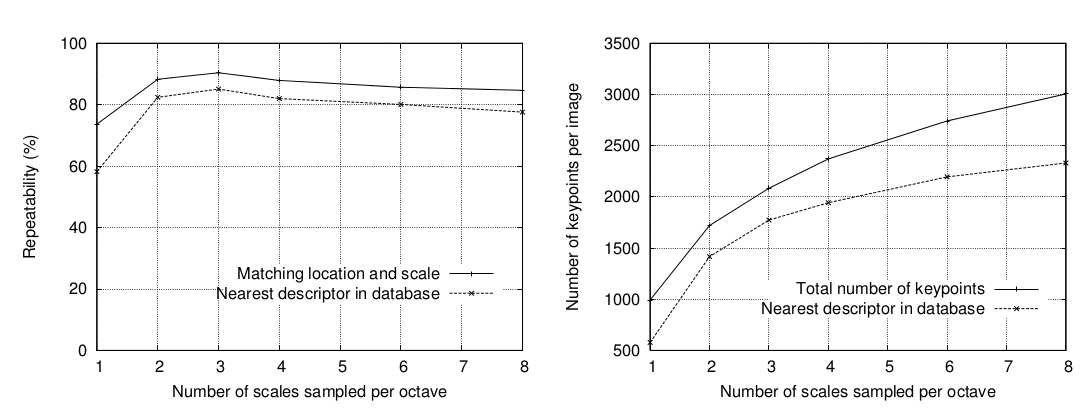
\includegraphics[width=0.6\textwidth]{scale_number.png}
\centering
\end{figure}
Nachdem die \Glspl{scale} der ersten \Gls{octave} berechnet wurden, wird das Bild mit dem doppelten Initialwert von $ \sigma $ runterskaliert in dem jedes zweite Pixel jeder Reihe und jeder Spalte beibehalten wird. Das erhaltene Bild ist der erste \Gls{scale} der nächsten \Gls{octave} aus dem die darauf folgenden wie zuvor erstellt werden.
In fig ist das Ergebnis dieses Vorgangs veranschaulicht.

\begin{figure}[h]
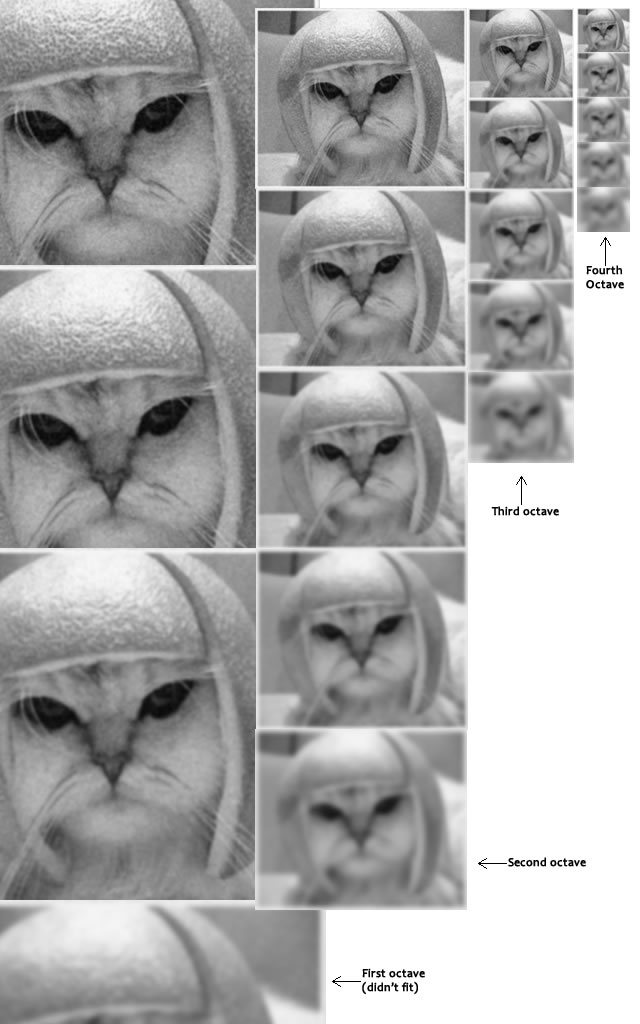
\includegraphics[width=0.4\textwidth]{sift-octaves.jpg}
\centering
\end{figure}

Um die Merkmale zu finden, werden die lokalen Extrema der \emph{Difference of Gaussian} Funktion zwischen den benachbarten \Glspl{scale} berechnet. Mikolajczyk fand in experimentellen Vergleichen mit anderen Bildfunktionen, wie der Gradient, die Hesse- und die Harrisfunktion, dass diese Methode die stabilsten Merkmale extrahiert.

Als erstes werden hierzu die \emph{Difference of Gaussian} zwischen den verschiedenen Ebenen des \Gls{scale-space}s ermittelt:	
\begin{equation}
D(x, y, \sigma) = (G(x, y, k\sigma) - G(x, y, \sigma)) \ast I(x, y)
= L(x, y, k\sigma) - L(x, y, \sigma)
\end{equation} 

Um die Lokalen Maxima zu finden, wird jedes Pixel mit den 8 benachbarten im selben \Gls{scale} und den 9 benachbarten in den darüber und darunter liegenden \Glspl{scale} verglichen. Stellt das Pixel ein Maximum oder ein Minimum in der betrachteten Menge von Pixeln da, stellt es einen potentiellen \emph{Keypoint} da.

\begin{figure}[h]
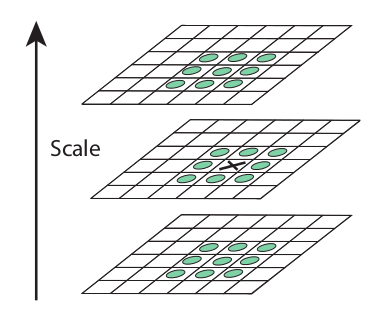
\includegraphics[width=0.4\textwidth]{sift_maxima.png}
\centering
\end{figure}

Um nur die stabilsten \emph{Keypoints} beizubehalten wurde von Brown vorgeschlagen mit Hilfe der quadratischen Taylorexpansion die Position der Keypoints auf Subpixel-Genauigkeit zu bestimmen.
Außerdem werden auch Keypoints mit einem niedrigen Kontrast gefiltert.

Da die Suche nach Keypoints mit der \emph{Difference of Gaussian} Funktion an den Kanten viele unsignifikante Punkte liefert werden anschließend die Gradienten der Punkte in x und y-Richung und deren Verhältnis $ r $ berechnet. Ist dieses größer als ein Schwellwert (Lowe verwendet r=10) wird der Keypoint gelöscht.

Um die Keypoints Rotationsinvariant zu machen wird ihnen eine Richtung zugewiesen. Lowe hat herausgefunden dass sich hierzu die Orientierung der Bildpunkte um den Keypoint gut eignet. 
Er berechnet die Größe und die Orientierung der Gradienten der umliegenden Pixel im \Gls{scale} des jeweiligen Keypoints:
\begin{equation}
m(x, y) = \sqrt{(L(x + 1, y) - L(x - 1, y))^{2} + (L(x, y + 1) - L(x, y - 1))^{2}}
\end{equation}
\begin{equation}
\Theta (x, y) = tan^{-1}((L(x, y + 1) - L(x, y - 1))/(L(x + 1, y) - L(x - 1, y)))
\end{equation}
Die Orientierungen werden anschließend mit den Größen gewichtet in 36 \"bins\" eines Histogramms unterteilt. Dem Keypoint wird die häufigste Orientierung des Histogramms zugewiesen und zusätzlich wird ein Keypoint mit jeder Orientierung die mindestens 80\% der maximalen Häufigkeit besitzt erstellt.

\subsection{Deskriptorberechnung}

Um die Keypoints zu charakterisieren wird ein sogenannter \emph{Deskriptor} berechnet.
Hierzu werden die Gradientengrößen und Orientierungen eines 16x16 Pixel Feldes um den Keypoint bestimmt und mit der Gaussfunktion gewichtet um den Einfluss entfernterer Punkte zu verringern.
Die Rotationsinvarianz des \emph{Deskriptors} wird erreicht in dem die Orientierungen der Gradienten relativ zur Orientierung des Keypoints gedreht werden.

\begin{figure}[h]
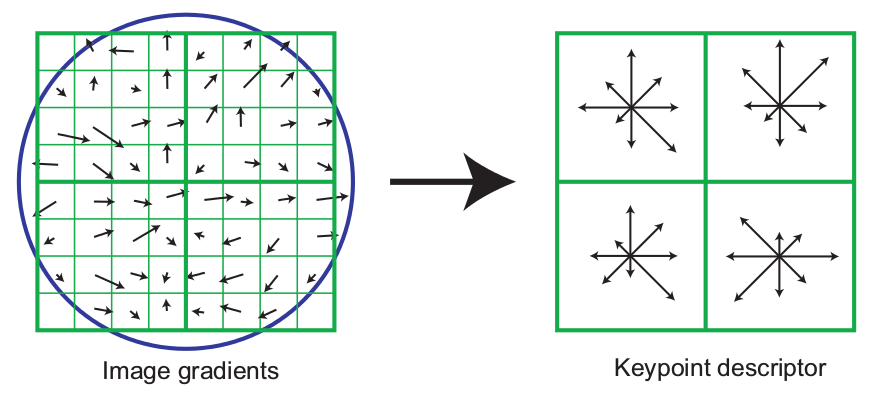
\includegraphics[width=0.8\textwidth]{sift_orientation.png}
\centering
\end{figure}

Die Pixel werden in 4x4 kleinere Felder unterteilt und innerhalb dieser werden wie bei der Orientierungsbestimmung der Keypoints die gewichteten Werte der Gradienten in Histogramme akkumuliert. Diese besitzen 8 \"bins\" die den Orientierungen entsprechen. Zusätzlich werden die Gradienten trilinear interpoliert indem sie nach einer Gewichtung in Abhängigkeit der Distanz auch auf die benachbarten Histogramme aufsummiert werden. Dadurch entsteht bei der Wiedererkennung der Merkmale ein bestimmtes Maß an Toleranz, dass die Erkennung von Objekten aus einem anderen Sichtwinkel oder nach einer nicht-starren Deformation ermöglicht.

Die \emph{Deskriptoren} werden als Vektoren gespeichert, die alle $4x4x8=128$ Werte der \"bins\" der Histogramme enthalten. 
Die Merkmale sind gegen Helligkeitsveränderungen die gleichermaßen alle Pixel aus denen sie berechnet wurden betreffen stabil, da die Gradienten durch Differenzen gebildet werden.
Um Stabilität gegen Kontrastveränderungen zu erreichen wird der Merkmalsvektor normiert.
Um den Einfluss von nicht linearen Helligkeitsveränderungen zu verringern werden alle Werte des Vektors die Größer als 0.2 sind auf diesen Wert gesetzt. Anschließend wird der Vektor nochmals normiert.


\section{SURF}

Nachdem es mit SIFT und anderen Algorithmen möglich war sehr charakterisierende und somit mit sehr hoher Wiederholgenauigkeit erkennbare Merkmale aus Bildern zu extrahieren, kam das Bedürfnis nach einer Lösung die weniger rechenintensiv ist auf um Merkmalserkennung auch in \Glspl{Online-System}n anzuwenden.
Mit diesem Ziel entwickelten H. Bay, T. Tuytelaars und L. Van Gool die \"Speeded Up Robust Features\", kurz SURF, und veröffentlichten diese im Jahr 2006.

\subsection{Merkmalsextraktion}

Der Detektor von SURF-Merkmalen basiert auf der Hesse-Matrix, diese enthält die zweiten Ableitungen der 2D-Gaussfunktion:
\begin{equation}
H(x, \sigma) =
\begin{bmatrix}
L_xx (x, \sigma) & L_xy (x, \sigma) \\
L_xy (x, \sigma) & L_yy (x, \sigma)
\end{bmatrix}
\end{equation}
Er benutzt die Determinante dieser um die Position und den Scale der Keypoints du detektieren.
Diese wird außerdem noch durch die Varianz der Gaussfunktion geteilt um das Ergebnis zu normalisieren:
\begin{equation}
DoH(x, y, \sigma)=\dfrac{G_{xx}(x, y, \sigma)\cdot G_{yy}(x, y, \sigma)-G_{xy}(x, y, \sigma)^{2}}{\sigma^{2}}
\end{equation}

Statt wie bei den SIFT-Merkmalen den Laplacian of Gaussian durch die Difference of Gaussian zu approximieren, verwenden die Autoren des SURF Verfahrens den Rechteck Filter.

\begin{figure}[h]
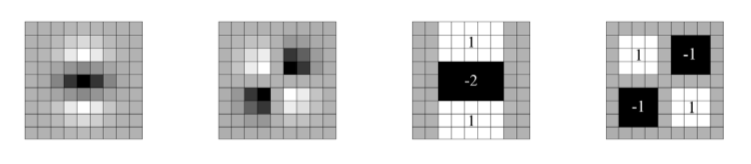
\includegraphics[width=0.9\textwidth]{surf_boxfilter.png}
\centering
\end{figure}

Dieser ist zwar nicht so genau, aber dafür durch die Benutzung von Integralbildern viel schneller zu berechnen.
Jede Position $X=(x, y)$ des Integralbildes stellt die Summe aller Pixel des durch die Position $X$ und den Ursprung aufgespannten Rechtecks:
\begin{equation}
I_\Sigma(X)=\sum_{i=0}^{i\leq x}\sum_{j=0}^{j\leq y}I(x,y)
\end{equation}

Ein weiterer Geschwindigkeitsvorteil wird dadurch erzielt dass der Scale-Space nicht im Voraus berechnet werden muss. Durch die Integralbilder sind die Kosten der Berechnung der Rechteckfilter nicht von der Größe der Maske abhängig und somit können die verschiedenen \Glspl{scale} durch die Anpassung der Maskengröße simuliert werden und das Originalbild muss für die verschiedenen \Glspl{octave} nicht mehr verkleinert werden.

\subsection{Deskriptorberechnung}

Der SURF Desktriptor ist von der Grundidee dem SIFT-Deskriptor sehr ähnlich.
Auch hier wird als erstes die Orientierung extrahiert und dann das Merkmal durch sein Umfeld charakterisiert.
Hierzu verwendet SURF allerdings Haar Wavelets da diese sehr schnell berechenbar sind.

Um die Orientierung zu bestimmen werden ein horizontales und ein vertikales Haar Wavelet (fig x) in einem Umkreis von $6s$ um das Merkmal in dem entsprechenden Scale $s$ des Merkmals berechnet.
Auch hier wird auf Integralbilder zurückgegriffen da die Wavelets eine Seitenlänge von $4s$ haben und somit für größere Scales sehr groß werden.
Der Umkreis des Merkmals wird in Abschnitte mit einer Breite von $\dfrac{\pi}{3}$ unterteilt und in jedem werden die Ergebisse des Horizontalen Wavelets und anschließend die des Vertikalen aufsummiert.
Somit erhält jeder Abschnitt ein Orientierungsvektor und der mit dem größten Betrag wird als Orientierung des Merkmals verwendet.

Um den Deskriptor zu extrahieren wird ein Quadrat mit $20s$ Seitenlänge, das nach der vorher bestimmten Orientierung ausgerichtet ist, um das Merkmal gespannt.
Dieses wird in 4 gleichgroße Unterbereiche unterteilt und in jedem dieser werden die Horizontalen und Vertikalen (in Bezug auf die Orientierung des Merkmals) Haar-Wavelets $d_x$ und $d_y$ für 5x5 gleichmäßig verteilte Punkte ermittelt. 
Die Ergebnisse der Haar-Wavelets werden dann aufsummiert und zusätzlich werden noch die Beträge der einzelnen Komponenten aufsummiert.
Hiermit erhält man einen vierdimensionalen Vektor für jeden der 16 Unterbereiche:
\begin{equation}
v=(\sum d_x, \sum d_y, \sum |d_x|, \sum |d_y|)
\end{equation}
Wie diese Methode eine Charakterisierende Beschreibung für das Umfeld eines Merkmals ist beschreiben die Autoren im folgenden Bild.

\begin{figure}[h]
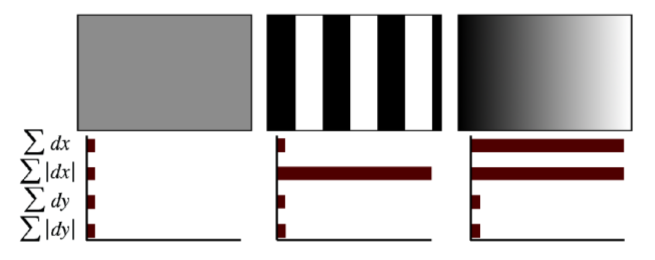
\includegraphics[width=0.8\textwidth]{surf_descriptor_expl.png}
\centering
\end{figure}

Wie auch der Merkmalsvektor bei SIFT, ist dieser bei SURF invariant gegenüber globalen Beleuchtungsveränderungen. Auch hier wird eine Kontrastinvarianz durch die Normierung erzielt.

\section{ORB}

Ein weiterer Algorithmus um effizient Merkmale aus Bildern zu extrahieren wurde von Edward Rosten und Tom Drummond unter dem Namen ORB vorgestellt.
ORB steht für \emph{Oriented FAST and Rotated BRIEF} da die Merkmalslokalisierung auf FAST basiert und die Deskriptorbeschreibung eine verbesserte Version von BRIEF ist.

\subsection{Merkmalsextraktion}
Um die Funktionsweise von Oriented FAST besser zu beschreiben wird im folgenden der darunterliegende Algorithmus FAST erläutert.
\subsubsection{FAST}

Der \emph{Features from Accelerated Segment Test} (FAST) ist vom Segment Test abgeleitet.

\begin{figure}[h]
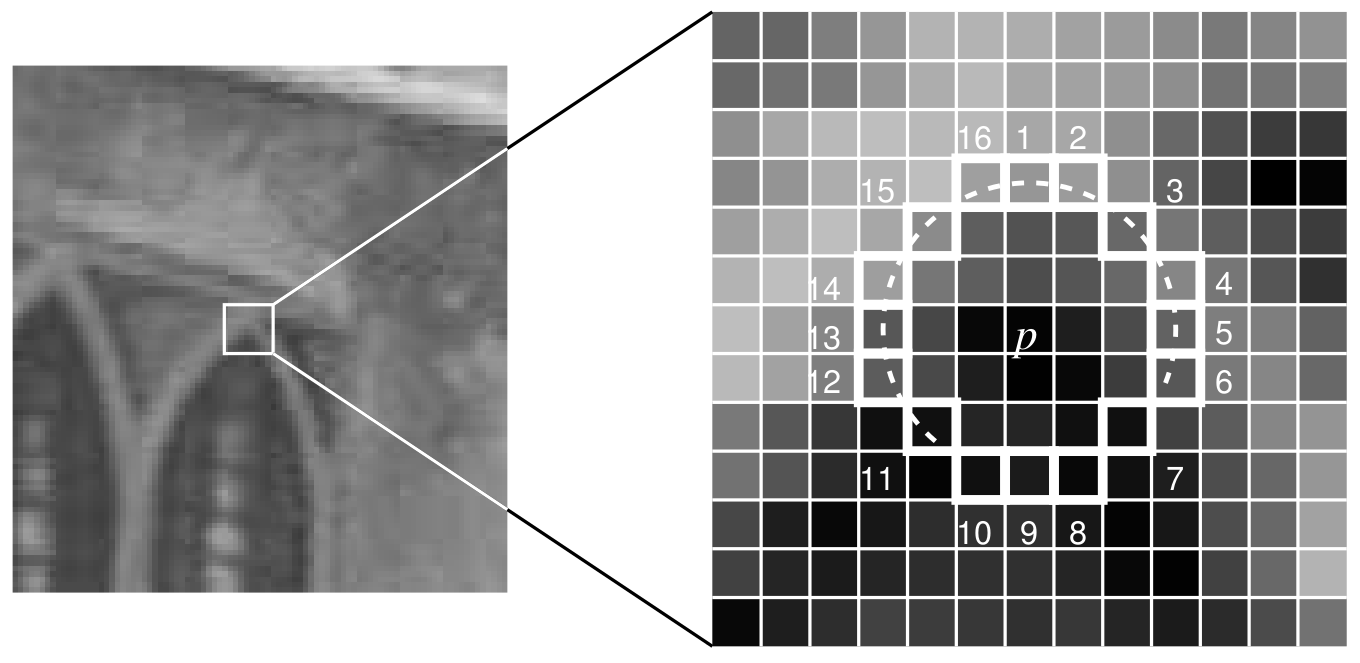
\includegraphics[width=0.8\textwidth]{segment_test.png}
\centering
\end{figure}

Dieser untersucht das Umfeld der einzelnen Punkte im Bild in dem er den umliegenden Kreis mit 16 Pixeln Länge mit dem Zentrum vergleicht.
Um möglichst schnell viele Bildpunkte raus zu filtern werden vorerst nur die Pixel 1, 5, 9 und 13 berücksichtigt und nur Punkte bei den 3 von diesen Pixeln heller oder dunkler als der berücksichtigte Bildpunkt sind als Kandidaten genommen.
Die Bildpunkte die den ersten Test bestehen werden anschließend genauer analysiert in dem jedes Pixel des umliegenden Kreises mit dem Zentrum verglichen wird.
Wenn der Kreis eine zusammenhängende Kette von Pixeln die heller oder dunkler als der zugehörige Bildpunkt sind beinhaltet, wird dieser als Merkmal hinterlegt.
Um diesen Vorgang zu optimieren wird bei FAST von maschinellem lernen gebrauch gemacht: es wird ein \emph{Decision Tree} wie von Quinlan in \emph{Induction of Decision Trees} beschrieben aufgebaut.
Um das System einzulernen wird ein Set aus Bildern genutzt, die bestenfalls dem Typ von Umgebung entsprechen in dem das Bildverarbeitungssystem benutzt werden soll.
Jedes Pixel dieser Bilder wird mit jedem Punkt $ x \in {1..16} $ des umliegenden Kreises verglichen um dann jedem Kreispunkt einen Zustand zuzuweisen:
\begin{equation}
S_{p\rightarrow x}=
\begin{cases}
d, & \quad I_{p\rightarrow x}\leq I_p - t\\
s, & \quad I_p - t < I_{p\rightarrow x} < I_p + t\\
b, & \quad I_p + t \leq I_{p\rightarrow x}
\end{cases}
\end{equation}
wobei $I_p$ die Intensität des Bildpunktes und $I_{p\rightarrow x}$ die Intensität des Pixels an der Stelle x auf dem Kreis um $I_p$ ist.
Anhand dieses Zustands werden alle Pixel $p$ der Menge $P$ aller Bildpunkte der Trainings-Bilder in die 3 Untermengen $P_d$, $P_s$ und $P_b$ unterteilt.
Um das $x$ zu bestimmen welches am aussage kräftigsten ist, wird die Entropie der Ecken-Eigenschaft $K$ (bei Pixeln  $p$ die als Ecke erkannt wurden hat $K_p$ den Wert 1) in den Mengen $P$,$P_d$, $P_s$ und $P_b$ berechnet.
Hieraus wird der Informationsgewinn berechnet als:
\begin{equation}
H(P) - H(P_d) - H(P_s) - H(P_b)
\end{equation}
Das $x$ mit dem höchsten Informationsgewinn wird zur Unterteilung von $P$ in seine Teilmengen verwendet.
Dieser Vorgang wird so lange wiederholt bis die Entropie einer der Untermengen zu $0$ wird und somit entweder nur oder keine Ecken enthält.
\subsubsection{Oriented FAST}
Da FAST keine Orientierungskomponente hat ist der Algorithmus nicht rotationsinvariant.
Um dieses Problem zu beheben wird von dem \emph{Intensitäts-Schwerpunkt} Gebrauch gemacht da dieser bei einer Ecke nie mit dem Mittelpunkt übereinstimmen sollte.
Dieser Schwerpunkt wird wie folgt berechnet:
\begin{equation}
C = (\dfrac{m_{10}}{m_{00}}, \dfrac{m_{01}}{m_{00}})
\end{equation}
mit den Momenten:
\begin{equation}
m_{pq} = \sum_{x,y}x^p y^q I(x,y)
\end{equation}

Dem Merkmal wird dann die Orientierung des Vektors der vom Mittelpunkt des Winkels $O=(0,0)$ zum \emph{Intesitäts-Schwerpunkt} zeigt zugewiesen:
\begin{equation}
\Theta = atan2(m_{01},m_{10})
\end{equation}

Um die Rotationsinvarianz zu optimieren, werden die Momente nur aus Pixeln berechnet deren x und y Werte innerhalb eines durch den Radius r um den Mittelpunkt aufgespannten Kreises liegen.

Bild Intensitätsschwerpunkt?


\subsection{Deskriptorberechnung}

\subsubsection{BRIEF}
BRIEF ist eine Methode zur Merkmalsextraktion die gegenüber SURF noch einen Schritt weiter in der Rechenzeitoptimierung geht. Hierzu verwenden die Authoren die Erkenntnisse der Arbeiten \emph{Fast Keypoint Recognition Using Random Ferns} und \emph{Keypoint Recognition Using Randomized Trees}.
Diese haben gezeigt das Teile eines Bildes effektiv durch wenige Vergleiche der Intensität in Pixelpaaren beschrieben werden können. 
Um einen BRIEF Deskriptor zu berechnen wird der folgende Test $\tau(p;x,y)$ auf die zu untersuchenden Pixelpaare angewandt und die Binären Ergebnisse in einem Vektor gespeichert:
\begin{equation}
\tau(p;x,y)=
\begin{cases}
1, & \quad \text{if } p(x) < p(y)\\
0, & \quad \text{otherwise}
\end{cases}
\end{equation}
Um die Störungsanfälligkeit zu reduzieren wird das Bild davor mit einem Gaussfilter geglättet.
Um den Filter effektiv zu nutzen haben die Autoren die drei Einflussgrößen experimentell bestimmt:
\begin{itemize}
\item \emph{Kernel des Gaussfilters}: Nachdem verschiedene Gausskurvenbreiten $\sigma$ zwischen 0 und 3 getestet wurden, hat sich $\sigma=2$ als die beste Wahl herausgestellt. Als Größe des Kernels wurde 9x9 Pixel genommen.

\item \emph{Räumliche Anordnung der Tests}: Wie die Versuche mit verschiedenen Strategien zur bestimmung der Anordnung der Tests gezeigt haben, spielt diese eine wichtige Rolle für die Güte (Wiedererkennungsrate) der Deskriptoren.
Folgende Anordnungen wurden verglichen:
\begin{figure}[h]
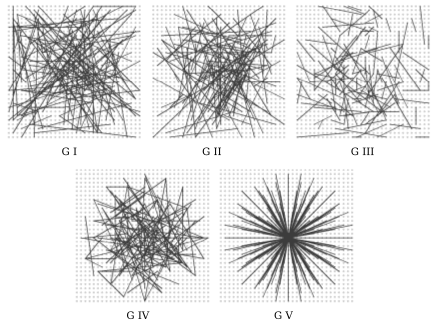
\includegraphics[width=0.6\textwidth]{brief_distribution.png}
\centering
\end{figure}

Die ergebnisse des Vergleichs sind im folgenden Graphen zu sehen:
\begin{figure}[h]
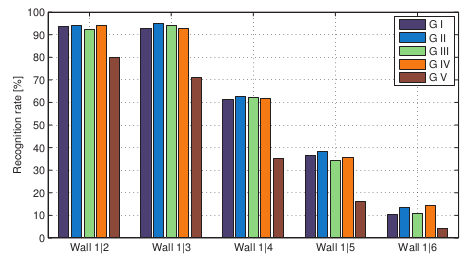
\includegraphics[width=0.6\textwidth]{brief_placement_results.png}
\centering
\end{figure}
Die symmetrische Anordnung ist klar die schlechteste und die Zweite ist in den meisten Fällen ein bisschen im Vorsprung gegenüber dem Rest, daher wird diese verwendet.
Es handelt sich hierbei um eine isotropische Gaussverteilung mit $\sigma^2=\frac{1}{25}S^2$ wobei $S$ die Seitenlänge des zu betrachtenden viereckigen Bildausschnitts ist.

\end{itemize}

\subsubsection{Rotated BRIEF}
BRIEF besitzt eine sehr schlechte Rotationsinvarianz, daher wurde für ORB die Variante Rotated BRIEF entworfen.
Für das Set aus Tests zur Erstellung des Deskriptorvektors an den stellen $(x_i, y_i)$ wird diese Matrix definiert:
\begin{equation}
S=
\begin{pmatrix}
x_1 & \cdots & x_n \\
y_1 & \cdots & y_n
\end{pmatrix}
\end{equation}

Anschließend wird die der $\Theta $ des Merkmals entsprechende Rotationsmatrix $R_\Theta$ verwendet um $S_\Theta $ wie folgt zu berechnen:
\begin{equation}
S_\Theta = R_\Theta \cdot S
\end{equation}
$\Theta$ wird auf Abschnitte mit einer Breite von $\dfrac{2\pi}{30}$ diskretisiert und es wird eine Lookup-Tabelle mit den Positionen der zu testenden Punkte für jeden Diskretisierungsschritt hinterlegt.
Somit lassen sich die rotationsunabhängigen Deskriptoren praktisch genauso schnell wie die rotationsabhängigen berechnen.
    \chapter{Merkmalsextraktion}

Um die verschiedenen Verfahren zur Merkmalsextraktion zu vergleichen wurde ein ein Programm in C++ erstellt.
Die genutzten Implementierungen der Bildverarbeitungsalgorithmen stammen aus der Bibliothek OpenCV. Hierbei handelt es sich um eine unter der BSD Lizenz veröffentlichten Software die sehr viele Methoden zur Bildverarbeitung und Maschinellem sehen enthält.
    \chapter{Ergebnisse}

\section{Laufzeit}


Um die verschiedenen Methoden zu vergleichen wurden verschiedene Tests durchgeführt.
Als erstes wurde die Laufzeit der einzelnen Verfahren verglichen. 
Hierzu wird von der \emph{clock\_gettime} Funktion gebraucht gemacht. Diese liefert einen \emph{struct} aus dem die zeit bis auf Nanosekunden-Genauigkeit ausgelesen werden kann.
Es wurden folgende Laufzeiten für jeden Algorithmus ermittelt:
\begin{itemize}
\item Extraktion der Merkmale
\item Matching der Deskriptoren
\item Berechnung der Homographie
\item Gesamte Bearbeitung eines Frames
\end{itemize}

Die für den ersten Punkt benötigte Zeit ist stark von der gewählten Methode abhängig. 
Die Matching-Zeit hängt zum einem von dem Deskriptortyp ab und zum anderen ist diese sehr von der Umgebung bestimmt da sie von der Anzahl der Merkmale abhängt.
Die Laufzeit der Homographie-Bestimmung hängt auch von der Merkmalsanzahl ab.

In Volgender Tabelle sind die Durchnittlichen Laufzeiten aufgelistet. Diese wurden bei der Bearbeitung eines Testvideos ermittelt.

\begin{center}
    \begin{tabular}{ c | C | C | C | C |}
      & Extraktion & Matching & Homographie & Gesamt\\ \hline
    SIFT & 370 & 90 & 2 & 495 \\ \hline
    SURF & 111 & 47 & 2 & 184 \\ \hline
    ORB & 17 & 25 & 6 & 64 \\
    \hline
    \end{tabular}
\end{center}


\section{Anzahl der korrekten Matches}

Als weiteres Testkriterium wurde die Anzahl der richtig zugewiesenen Merkmale bestimmt.
Hierzu wurde von der Bitmaske die von \emph{findHomography} zurückgegeben wird Gebrauch gemacht. Aus dieser können die tatsächlich von der Funktion verwendeten Matches bestimmt werden. Die gefundenen Matches passen somit in die Gesamtkonstellation und werden als richtig eingestuft.
Um möglichst aussagekräftige Ergebnisse zu erhalten wurden 40 sekündige Videos der Testobjekte aufgenommen und anschließend die durchschnittlichen Korrekten Matches für jeden Algorithmus berechnet. Um unvorhersehbare Effekte beim Startvorgang des Programms auszuschließen wurden für die Mittelwerte nur Matches ab der 10. Sekunde berücksichtigt.


\begin{center}
    \begin{tabular}{ c | C | C | C | C | C |}
      & Kork & Müsli & Tomatendose & Kirschglas & Spardose \\ \hline
    SIFT & 80 & 298 & 181 & 161 & 46 \\ \hline
    SURF & 11 & 149 & 80 & 78 & 17 \\ \hline
    ORB & 26 & 156 & 110 & 170 & 59 \\
    \hline
    \end{tabular}
\end{center}

Wie erwartet schneiden die Merkmale die von einem SIFT-Deskriptor beschrieben werden bei der Wiedererkennung am besten ab.
Bei 3 von den 5 Testobjekten werden deutlich mehr Merkmale korrekt wiedererkannt als bei den anderen beiden Methoden.
Allerdings werden bei den schwerer zu erkennenden Objekten anhand des ORB-Deskriptors mehr Merkmale richtig zugeordnet.
SURF liefert in diesem Test für alle 5 Objekte das schlechteste Ergebnis.

\section{Stabilität gegen Rotation}

Beim zweiten Vergleich wurde getestet wie rotationsinvariant die Algorithmen sind.
Hierzu wurde jedes Objekt soweit gedreht bis keine eindeutige Lokalisierung mehr möglich war.
Hierbei wurde darauf geachtet dass bei den Vergleichen die Position der Kamera konstant blieb und die Objekte nur um ihre senkrechte Achse gedreht wurden.
Nachdem die maximale Rotation erreicht wurde, wurde der Winkel gemessen und auf 5 Grad gerundet, da eine genauere Messung mit den vorhandenen Mitteln nicht möglich war.

\begin{center}
    \begin{tabular}{ c | C | C | C | C | C |}
      & Kork & Müsli & Tomatendose & Kirschglas & Spardose \\ \hline
    SIFT & 55 & 60 & 55 & 65 & 35 \\ \hline
    SURF & 45 & 55 & 50 & 45 & 35 \\ \hline
    ORB & 45 & 45 & 30 & 55 & 25 \\
    \hline
    \end{tabular}
\end{center}

Auch hier liefert SIFT die besten Ergebnisse, selbst bei den schwerer zu erkennenden Objekten, obwohl bei diesen weniger Merkmale als bei ORB korrekt zugeordnet wurden.
Auch SURF ist trotz der wesentlich geringeren Menge an Merkmalen im schnitt besser als ORB.

\section{Stabilität gegen Skalierung}

Eine weitere wichtige Eigenschaft der Merkmale ist die Skalierungsinvarianz.
Diese führt dazu dass Objekte auch erkannt werden wenn sie kleiner oder größer (weiter oder weniger weit entfernt) als auf dem Modellbild sind.
Da die SURF und ORB Implementierungen von OpenCV nicht mit kleinen Bildern funktionieren, und die Modellbilder somit nicht runterskaliert werden konnten, war es nicht möglich die Erkennung von Objekten die größer als ihr Modellbild sind zu testen.
Da in der Praxis die zu erkennenden Objekte aber kleiner als deren Modellbilder sind, stellt dies aber kein wirkliches Problem da.
Um die Algorithmen auf die Fähigkeit kleinere Exemplare der Ojekte wiederzuerkennen zu testen, wurde die maximale Distanz von der Kamera zum Objekt gemessen bei der dieses noch korrekt erkannt werden konnte.

\begin{center}
    \begin{tabular}{ c | C | C | C | C | C |}
      & Kork & Müsli & Tomatendose & Kirschglas & Spardose \\ \hline
    SIFT & 50 & 265 & 120 & 110 & 70 \\ \hline
    SURF & 25 & 140 & 65 & 70 & 50 \\ \hline
    ORB & 30 & 125 & 45 & 50 & 40 \\
    \hline
    \end{tabular}
\end{center}

Wie bei den vorherigen Tests schnitt SIFT mit Abstand am besten ab und schaffte es, für die Verhältnisse (Consumer Grade Webcam mit VGA Auflösung), Objekte aus einer sehr großen Entfernung zu erkennen.
SURF schnitt bei allen Objekten außer dem Korkuntersetzter besser als ORB ab.

\section{Stabilität der Lokalisierung}

Ein weiteres Maß für die Güte der verschiedenen Extraktionsverfahren ist die Abweichung der Lokalisierung von der Istposition der Objekte.
Genauer ist hier die quadratische mittlere Abweichung, die Varianz, von Bedeutung.
Um diese zu ermitteln wurde auch hier ein Testvideo erstellt um gleiche Bedingungen zu gewährleisten.
Es wurde ein Histogramm von der Verteilung der X-Koordinate, der Y-Koordinate und dem Ausrichtungswinkel in Form eines Vectors erstellt.
Die als \emph{•}{csv}-Datei aus dem Programm exportierten Daten wurden mittels Gnuplot als Graphen dargestellt.
Die Verteilungen sind in den folgenden drei Graphen zu sehen, hierbei ist links die Rotation zu sehen und rechts davon die Trasnlation in x und y Richtung.
Die Translation ist jeweils in Pixeln angegeben, dies ist auch die Einheit der Zahlen auf den Achsen.
Die Rotation ist hingegen in Grad bemessen und wurde im Vergleich der angeschriebenen Zahlen gestreckt.

\begin{center}
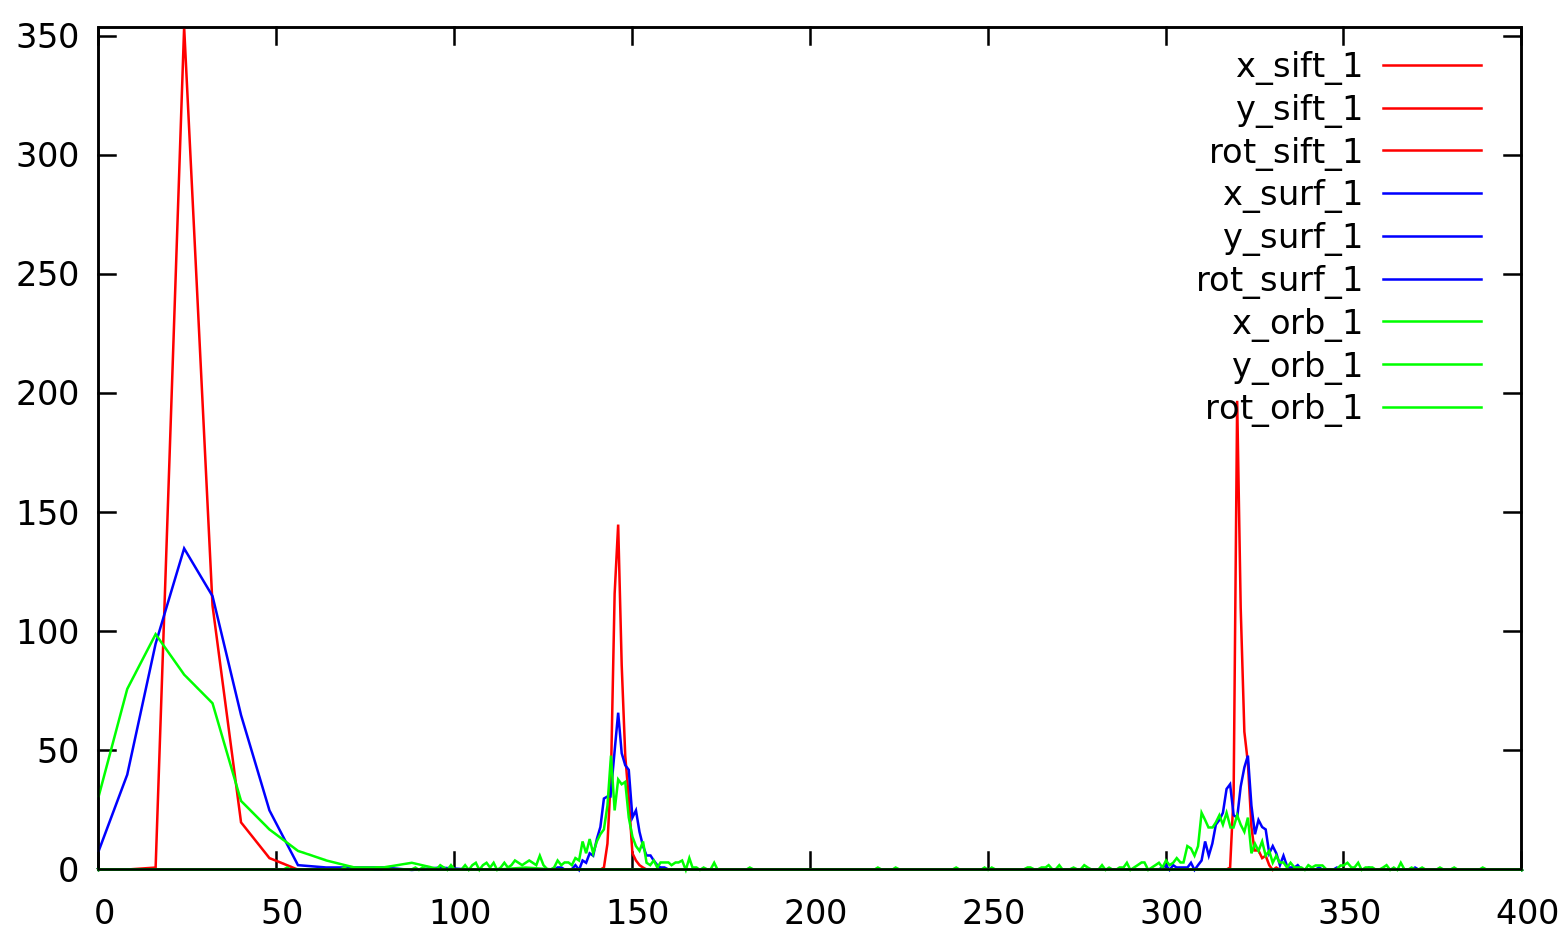
\includegraphics[width=0.75\textwidth]{verteilung1.png}

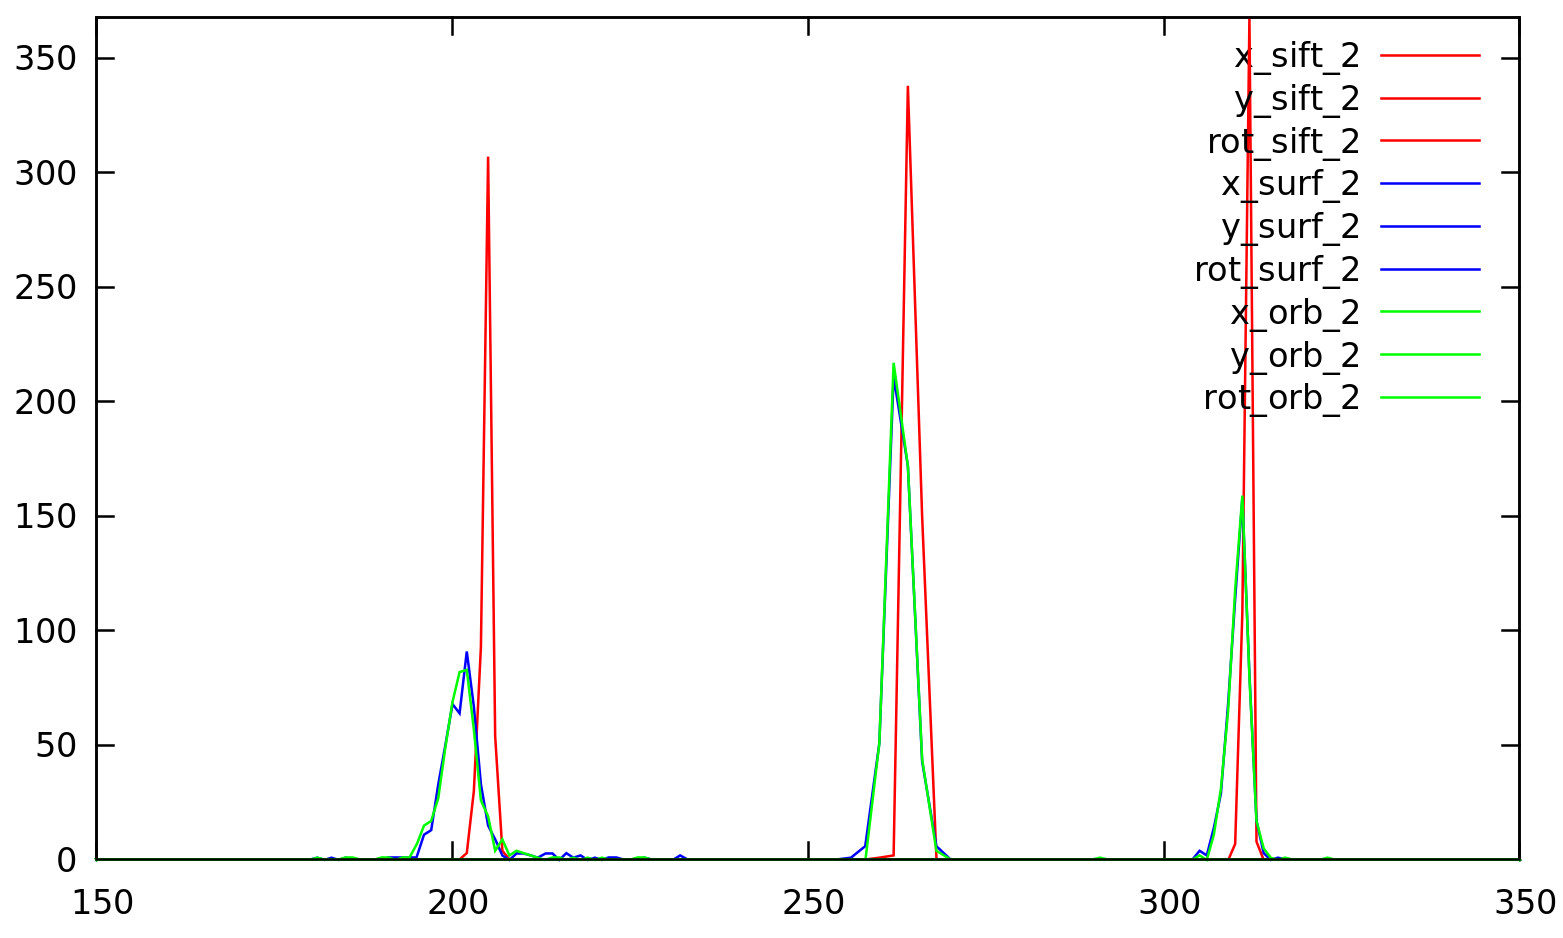
\includegraphics[width=0.75\textwidth]{verteilung2.png}

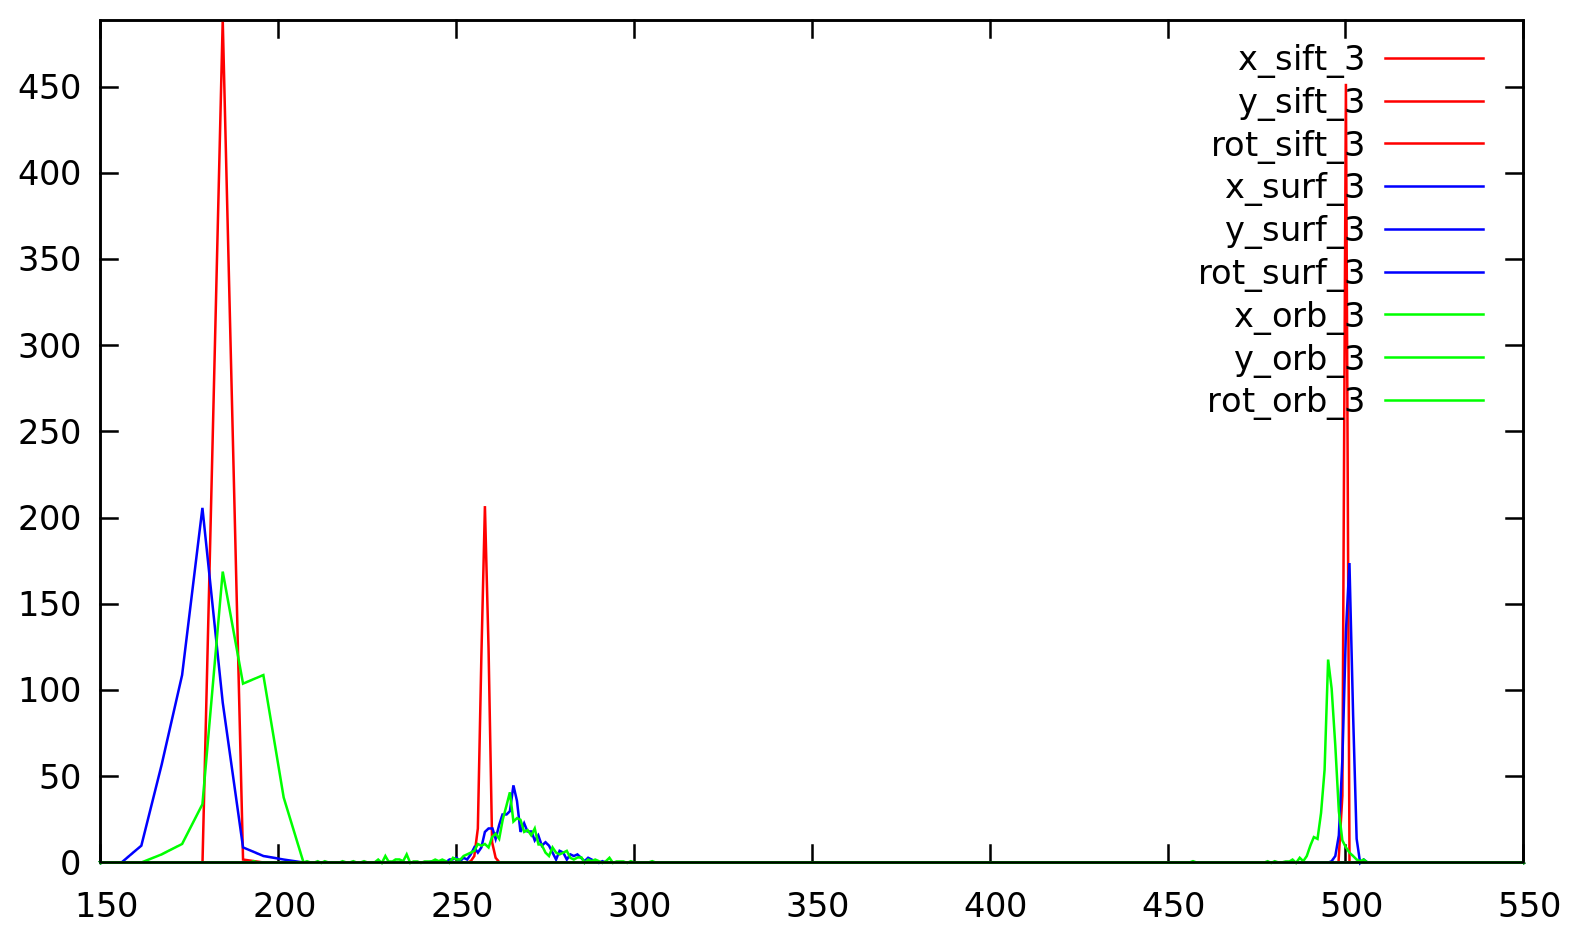
\includegraphics[width=0.75\textwidth]{verteilung3.png}
\end{center}


Wie zu erwarten da dies auch anhand der Videoausgabe des Programms deutlich sichtbar ist, zeigen die Graphiken deutlich dass die Lokalisierung durch den SIFT Algorithmus wesentlich stabiler als bei den anderen beiden Varianten ist.
SURF lokalisiert die Objekte mit größerer Genauigkeit als ORB, hat hierbei aber nur einen mäßigen Vorteil.
Man sieht dass die Verteilungen in Einigen Fällen einer summe mehrerer Normalverteilungen entsprechen. 
Dies kommt daher dass mehr als eine Konstellation an Merkmalen dem Modell ähnlich sind und somit durch die Störeinflüsse manchmal eine vollkommen falsche Position ausgegeben wird.

\section{Testvideos}

Der letzte Vergleich wurde anhand von zwei Testvideos gemacht.
Diese beinhalten die 5 Beispielgegestände in zwei verschiedenen Anordnungen.
Die Leistung der 3 Algorithmen wurde die Anzahl der Frames in welchen die Objekte erkannt wurden bestimmt.
Da es bei der gleichzeitigen Verwendung von mehreren Objekten leichter zu Fehlerkennungen kommt wurden nur Frames in denen ein Objekt mit mindestens 5 Matches erkannt wurde gezählt. 
Dies führt dazu dass es zu so gut wie keiner Fehlzuweisung kommt (weniger als 5 pro Video beobachtbar).
In folgender Tabelle sind die Anzahlen der Frames des ersten Testvideos in denen die jeweiligen Objekte gefunden wurden aufgelistet:

\begin{center}
    \begin{tabular}{ c | C | C | C | C | C |}
      & Kork & Müsli & Tomatendose & Kirschglas & Spardose \\ \hline
    SIFT & 268 & 415 & 392 & 212 & 203 \\ \hline
    SURF & x & 400 & 366 & 162 & 77 \\ \hline
    ORB & x & 370 & 342 & 150 & 56 \\
    \hline
    \end{tabular}
\end{center}

Es folgen die Frames des zweiten Videos:

\begin{center}
    \begin{tabular}{ c | C | C | C | C | C |}
      & Kork & Müsli & Tomatendose & Kirschglas & Spardose \\ \hline
    SIFT & 300 & 793 & 517 & 669 & 696 \\ \hline
    SURF & x & 695 & 285 & 548 & 443 \\ \hline
    ORB & 2 & 531 & 123 & 341 & 114 \\
    \hline
    \end{tabular}
\end{center}

Zusätzlich wurden die durchschnittlichen Zuweisungen die zu der Erkennung der Objekte geführt haben berechnet.
Erstes Video:

\begin{center}
    \begin{tabular}{ c | C | C | C | C | C |}
      & Kork & Müsli & Tomatendose & Kirschglas & Spardose \\ \hline
    SIFT & 17 & 124 & 40 & 31 & 11 \\ \hline
    SURF & x & 48 & 10 & 10 & 5 \\ \hline
    ORB & x & 66 & 11 & 11 & 9 \\
    \hline
    \end{tabular}
\end{center}

Zweites Video:

\begin{center}
    \begin{tabular}{ c | C | C | C | C | C |}
      & Kork & Müsli & Tomatendose & Kirschglas & Spardose \\ \hline
    SIFT & 9 & 65 & 22 & 44 & 26 \\ \hline
    SURF & x & 20 & 7 & 13 & 11 \\ \hline
    ORB & 6 & 23 & 9 & 14 & 18 \\
    \hline
    \end{tabular}
\end{center}

Wie nach den vorherigen Tests zu erwarten, stellte sich auch hier SIFT als der Beste Merkmalsextrahierungsalgorithmus heraus.
SURF extrahierte wie in einem der vorangegangenen Tests weniger Merkmale als ORB, schaffte es aber trotzdem die Objekte besser zu detektieren als ORB.
Das ist eine Folge der eindeutigeren Beschreibung der Keypoints durch den SURF-Deskriptor.
Der große Vorteil von SIFT gegenüber den anderen beiden Verfahren ist hierbei nicht nur dass die Objekte öfter erkannt werden sondern auch die Stabilität der Detektion.
Hierdurch lässt sich in einer wie in den Testvideos dargestellte Umgebung auch die Orientierung der Objekte mit sehr guter Annäherung bestimmen, während SURF und ORB hier eher nur zur Positionsbestimmung des Mittelpunktes der Objekte geeignet sind.
    \chapter{Ausblick}

Die Ergebnisse zeigen dass sich die untersuchten Algorithmen zufriedenstellend für die Klassifizierung von bekannten Objekten eignen.
Um diese aber mit genügender Genauigkeit zu lokalisieren sind zumindest SURF und ORB nicht ausreichend.
Auch mit SIFT wird in manchen Situationen die Orientierung der Objekte nicht genau erkannt.
Um die Detektion und die Lokalisierung der Objekte zu stabilisieren könnte ein Kalman-Filter implementiert werden.
Dieser verwendet ein Bewegungsmodell welches von der Natur der Objekte und/oder der Bewegung der Kamera abhängt.
Im Zusammenspiel mit den Messungen der Position durch den in dieser Arbeit beschriebenen Prozess und der zu erwartenden Ungenauigkeit schätzt der Filter die aktuelle Position der Objekte.
Dies hat den Vorteil dass das Ergebnis nicht nur von der aktuellen Messung sondern auch von den vorherigen abhängt und somit das Rauschen der Messungen kompensiert werden kann.


    \chapter{Zusammenfassung}

In dieser Arbeit wurden drei der meist verbreiteten Merkmalsextraktionsverfahren in einem Programm implementiert um sie untereinander zu vergleichen.
Die drei Algorithmen weisen jeweils Stärken und Schwächen auf.
Die Güte der Merkmale ist bei SIFT unter jedem Aspekt mit Abstand am besten.
Der Schwachpunkt dieses Verfahrens ist allerdings die Performance 

    \begin{appendix}
    %%=====================
\chapter{Hilfreiche Erkenntnisse für die weitere Softwareentwicklung}\label{app_1}
%=====================
\section{Debugging}
\label{debug}
%=====================
Debugging ist einer der teuersten Schritte in der Softwareentwicklung und nimmt einen Großteil der Kosten ein, die die Entwicklung kosten.

Unter diesem Aspekt habe ich die im ROS-Framework implementierte \quotes{rosconsle} sehr zu schätzen gelernt.
Sie bietet ein umfangreiches Set an Nachrichten-Levels (\quotes{verbosity}).

\begin{table}
\begin{center}
\begin{tabular}{p{3cm}  p{10cm}}
\textbf{Level} & \textbf{Beschreibung} \\ \hline	
	DEBUG & Nachrichten, die man nie sehen muss, wenn das Programm ordnungsgemäß läuft  \\ \hline
	INFO & Kleine Mengen an Informationen, die für den Anwender nützlich sind \\ \hline
	WARN & Informationen, die den Nutzer beunruhigen und die Ausgabe des Programms verändern können, aber im erwarteten Rahmen der Programmfunktion liegen \\ \hline
	ERROR & Ein ernster Fehler ist aufgetreten, aber das System kann sich von dem Fehler wieder erholen \\ \hline
	FATAL & Ein ernster Fehler ist aufgetreten und die Funktion kann nicht wiederhergestellt werden \\ 

\end{tabular}
\end{center}
\caption{\label{debugVerbosity}In der Tabelle werden die verschieden Debug-Levels beschrieben }
\end{table}
Ein weiteren Vorteil bringen benannte Logger-Nachrichten. 
Damit kann man später Filter einrichten. 
Am besten sieht man es am Beispiel:

\begin{verbatim}
ROS_DEBUG_NAMED_STREAM("task.step","Value is:"<<x);
\end{verbatim}


    \end{appendix}

    \backmatter
    \listoffigures
    \printnoidxglossaries
    \bibliographystyle{gerapali}    % für engl. Versionen nur "apalike", deutsch: gerapali plus package "bibgerm" im DA-style-File!
    \addcontentsline{toc}{chapter}{\bibname}
    
    \inputthesen

\end{document}
